%% meeting_update.tex
%% Compile with: pdflatex meeting_update.tex
\documentclass[11pt]{article}

\usepackage[margin=1.1in]{geometry}
\usepackage{amsmath, amssymb, amsthm}
\usepackage{mathtools}
\usepackage{booktabs}
\usepackage{array}
\usepackage{xcolor}
\usepackage{tikz}
\usetikzlibrary{arrows.meta, positioning, calc, shapes.geometric}
\usepackage{hyperref}
\hypersetup{colorlinks=true, linkcolor=blue!60!black, urlcolor=blue!60!black}

\newcommand{\R}{\mathbb{R}}
\newcommand{\dx}{\,dx}
\newcommand{\dt}{\,dt}
\newcommand{\half}{\tfrac{1}{2}}
\newcommand{\rhoO}{\rho_0}
\newcommand{\rhoT}{\rho_1}
% Laplacian notation (easily extended to multiple spatial dimensions)
\newcommand{\Dx}{\Delta_x}          % spatial Laplacian
\newcommand{\Dxt}{\Delta_{xt}}      % space-time Laplacian  partial_tt + Delta_x
\DeclareMathOperator{\prox}{prox}
\DeclareMathOperator{\proj}{proj}

\title{\textbf{Schr\"odinger Bridge / Dynamic Optimal Transport in 1D}\\[4pt]
       \large Problem Setup, Discretization, and ADMM Algorithm}
\author{}
\date{\today}

\begin{document}
\maketitle
\tableofcontents
\bigskip

% ============================================================
\section{Problem Setup}
% ============================================================

\subsection{Continuous Formulation (Benam\^ou--Brenier)}

We seek a curve of probability densities $\rho(t,x)$ and a momentum field
$m(t,x)$ on the space-time domain $[0,1]\times[0,1]$ solving the
\emph{dynamic optimal transport} problem:
%
\begin{equation}\label{eq:ot}
\min_{\rho,\, m} \int_0^1\!\int_0^1
    \frac{m(t,x)^2}{2\,\rho(t,x)} \dx\dt
\end{equation}
%
subject to the \textbf{continuity equation}
\begin{align}
  \partial_t \rho + \partial_x m &= 0,
    \label{eq:cont}\\
  \rho(0,\cdot) = \rhoO,\quad
  \rho(1,\cdot) &= \rhoT,
    \label{eq:bc_t}\\
  m(t,0) = m(t,1) &= 0,
    \label{eq:bc_x}\\
  \rho &\geq 0.
    \label{eq:pos}
\end{align}
%
The integrand $m^2/(2\rho)$ is the \emph{kinetic energy density}.
At the optimum the objective equals $W_2(\rhoO,\rhoT)^2$, the squared
2-Wasserstein distance.

\subsection{Regularization (Schr\"odinger Bridge)}

A diffusion coefficient $\varepsilon \geq 0$ replaces the continuity
constraint with the \emph{Fokker--Planck equation}:
\begin{equation}\label{eq:fp}
  \partial_t \rho + \partial_x m = \varepsilon\,\Dx\rho.
\end{equation}
As $\varepsilon\to 0$ the problem reduces to unregularized $W_2$ transport.
Positive $\varepsilon$ connects to the \textbf{Schr\"odinger bridge} problem
and smooths the solution, aiding numerics.

% ============================================================
\section{Staggered Grid Discretization}\label{sec:disc}
% ============================================================

\subsection{Grid Parameters}

\begin{center}
\begin{tabular}{lll}
\toprule
Symbol & Value & Meaning\\
\midrule
$N_x$ & user-set & number of spatial cells\\
$N_t$ & user-set & number of temporal slabs\\
$\Delta x$ & $1/N_x$ & spatial cell width\\
$\Delta t$ & $1/N_t$ & temporal slab height\\
\bottomrule
\end{tabular}
\end{center}

\subsection{Variable Locations}

Different unknowns live at \emph{different grid locations}
(MAC / staggered layout), which ensures exact discrete conservation:

\begin{center}
\begin{tabular}{llll}
\toprule
Variable & Time location & Space location & Array size\\
\midrule
$\rho$ & interior time faces $t_k = k\Delta t$ & cell centres & $(N_t-1)\times N_x$\\
$m$ & time cell centres $t_{k+\frac{1}{2}}$ & interior space faces & $N_t\times(N_x-1)$\\
\bottomrule
\end{tabular}
\end{center}

Boundary data $\rho(0,\cdot)=\rhoO$ and $\rho(1,\cdot)=\rhoT$ are held
fixed; the spatial boundary momenta $m(\cdot,0)=m(\cdot,1)=0$ are enforced
by restricting to interior faces only.

\subsection{Space-Time Grid Diagram}

\begin{center}
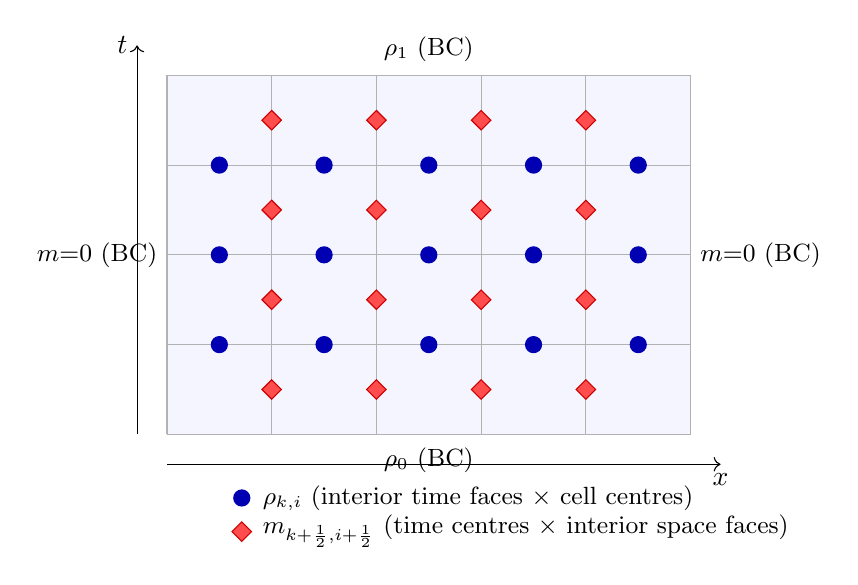
\begin{tikzpicture}[scale=0.95]
  % parameters
  \def\nx{5}  \def\nt{4}
  \def\dx{1.4} \def\dt{1.2}

  % shading for cell interiors
  \foreach \i in {0,...,3}{
    \foreach \j in {0,...,4}{
      \fill[blue!4] (\j*\dx,\i*\dt) rectangle (\j*\dx+\dx,\i*\dt+\dt);
    }
  }

  % vertical grid lines (spatial faces)
  \foreach \j in {0,...,5}{
    \draw[gray!60] (\j*\dx, 0) -- (\j*\dx, 4*\dt);
  }
  % horizontal grid lines (temporal faces)
  \foreach \i in {0,...,4}{
    \draw[gray!60] (0, \i*\dt) -- (5*\dx, \i*\dt);
  }

  % --- rho nodes: interior time faces x cell centres
  \foreach \i in {1,...,3}{       % interior time faces
    \foreach \j in {0,...,4}{     % cell centres
      \node[circle, fill=blue!70!black, inner sep=2.2pt]
        at (\j*\dx+0.5*\dx, \i*\dt) {};
    }
  }

  % --- m nodes: time cell centres x interior space faces
  \foreach \i in {0,...,3}{       % time cell centres
    \foreach \j in {1,...,4}{     % interior space faces
      \node[diamond, fill=red!70, inner sep=1.8pt, draw=red!80!black]
        at (\j*\dx, \i*\dt+0.5*\dt) {};
    }
  }

  % BC labels
  \node[above, font=\small] at (2.5*\dx, 4*\dt+0.05) {$\rho_1$ (BC)};
  \node[below, font=\small] at (2.5*\dx, -0.05) {$\rho_0$ (BC)};
  \node[left,  font=\small] at (0, 2*\dt) {$m{=}0$ (BC)};
  \node[right, font=\small] at (5*\dx, 2*\dt) {$m{=}0$ (BC)};

  % axis labels
  \draw[->] (-0.4,0) -- (-0.4, 4*\dt+0.4) node[left]{$t$};
  \draw[->] (0,-0.4) -- (5*\dx+0.4,-0.4) node[below]{$x$};

  % legend
  \node[circle, fill=blue!70!black, inner sep=2.2pt] at (1.0, -0.85) {};
  \node[right, font=\small] at (1.15,-0.85) {$\rho_{k,i}$\ (interior time faces $\times$ cell centres)};
  \node[diamond, fill=red!70, inner sep=1.8pt, draw=red!80!black] at (1.0,-1.3) {};
  \node[right, font=\small] at (1.15,-1.3) {$m_{k+\frac{1}{2},i+\frac{1}{2}}$\ (time centres $\times$ interior space faces)};
\end{tikzpicture}
\end{center}

\subsection{Finite Difference Operators}

Four first-order stencils cover the two directions and two grid offsets.
Below $D_t^\phi$ denotes the time derivative whose output sits at
\emph{time-face} locations (used in the continuity equation):
%
\begin{equation}
  (D_t^\phi\,\rho)_{k} = \frac{\rho_{k} - \rho_{k-1}}{\Delta t},
  \qquad k=1,\ldots,N_t-1,
\end{equation}
%
with boundary values $\rho_0 = \rhoO$ and $\rho_{N_t} = \rhoT$.
The transpose $D_t^\rho = -(D_t^\phi)^\top$ maps from faces to cell centres.
Analogous operators $D_x^\phi$ and $D_x^m$ act in the spatial direction.

The \textbf{discrete continuity equation} at each space-time cell $(k,j)$ is:
\begin{equation}\label{eq:disc_cont}
  \frac{\rho_{k+1,j} - \rho_{k,j}}{\Delta t}
  + \frac{m_{k+\frac{1}{2},j+\frac{1}{2}} - m_{k+\frac{1}{2},j-\frac{1}{2}}}{\Delta x} = 0.
\end{equation}

\subsection{Interpolation Operators}

Because $m^2/\rho$ couples variables at different locations, we define
second-order averaging operators:
%
\begin{equation}
  (I_t^\phi\,\rho)_k = \tfrac{1}{2}(\rho_{k-\frac{1}{2}} + \rho_{k+\frac{1}{2}}),
  \qquad
  (I_x^\phi\,m)_j = \tfrac{1}{2}(m_{j-\frac{1}{2}} + m_{j+\frac{1}{2}}),
\end{equation}
%
bringing both fields to the space-time \textbf{cell centres} where the
kinetic energy is evaluated.

\textbf{Adjoint note:} When the forward operator is affine,
$L(u) = Au + b$ (with $b$ encoding BCs), the adjoint is $L^*(v)=A^\top v$
--- the BC term is \emph{not} included. Using non-zero BCs in the adjoint
corrupts the gradient direction and leads to incorrect solutions.

\subsection{Fast Poisson Solve via DCT}

The projection step requires inverting the operator
$(-\Dxt + \varepsilon^2\Dx^2)$ with Neumann BCs, where
$\Dxt = \partial_{tt}+\Dx$ is the space-time Laplacian and
$\Dx^2$ is the spatial biharmonic.
Because the discrete Neumann Laplacian diagonalises in the DCT basis, the
eigenvalues are precomputed once:
%
\begin{align}
  \lambda_x^\ell &= \frac{2 - 2\cos(\pi\Delta x\,\ell)}{\Delta x^2},
    \quad \ell=0,\ldots,N_x-1, \label{eq:lx}\\
  \lambda_t^k    &= \frac{2 - 2\cos(\pi\Delta t\,k)}{\Delta t^2},
    \quad k=0,\ldots,N_t-1, \label{eq:lt}\\
  \lambda^{k,\ell} &= \lambda_t^k + \lambda_x^\ell
                      + \varepsilon^2\,(\lambda_x^\ell)^2.
    \label{eq:lbih}
\end{align}
%
The solve $\hat\phi = \widehat{\text{RHS}}\,/\,\lambda$ is $O(N_xN_t\log N_xN_t)$,
and the zero-mode $\lambda^{0,0}=0$ is handled by setting $\hat\phi^{0,0}=0$
(fixing the additive gauge of $\phi$).

% ============================================================
\section{ADMM Algorithm}
% ============================================================

\textbf{Optimize-first philosophy.}
ADMM is applied directly to the \emph{continuous} (infinite-dimensional)
Benamou--Brenier problem \eqref{eq:ot}--\eqref{eq:fp}.
The three ADMM steps --- proximal map, projection, and dual update ---
are derived in the continuous function-space setting.
Only afterwards is each step independently discretized onto the staggered
grid of Section~\ref{sec:disc}.
This \emph{optimize-first, discretize-second} ordering means the discrete
iteration does not fit the standard finite-dimensional ADMM framework, and
we currently have no formal convergence guarantee; convergence is
monitored empirically via the residual \eqref{eq:res}.

\subsection{Splitting Formulation}

We introduce an auxiliary copy $(\tilde\rho, \bar{m})$ of the primal
variables and rewrite \eqref{eq:ot}--\eqref{eq:fp} as the split problem
%
\begin{equation}
  \min_{\rho,m,\,\tilde\rho,\bar m}
  \underbrace{\int_0^1\!\int_0^1 \frac{m^2}{2\,\rho}\dx\dt}_{f(\rho,m)}
  + \underbrace{\iota_{\mathcal{C}}(\tilde\rho,\bar m)}_{g(\tilde\rho,\bar m)}
  \quad\text{s.t.}\quad
  (\rho,m)=(\tilde\rho,\bar m),
\end{equation}
%
where $\mathcal{C}$ is the \emph{continuous} Fokker--Planck constraint set:
\begin{equation*}
  \mathcal{C} = \bigl\{(\rho,m) :
    \partial_t\rho + \partial_x m = \varepsilon\,\Dx\rho,\;
    \rho(0,\cdot)=\rhoO,\;
    \rho(1,\cdot)=\rhoT,\;
    m(\cdot,0)=m(\cdot,1)=0
  \bigr\}.
\end{equation*}
Each ADMM step below is derived for this continuous problem and then
discretized independently.

\subsection{Iteration}

With penalty parameter $\gamma>0$ and dual variables $(\delta_\rho,\delta_m)$,
the three steps per iteration are:

\paragraph{Step 1 -- Proximal step (kinetic energy).}
\begin{equation}\label{eq:prox}
  (\rho^{n+1},m^{n+1}) \leftarrow
  \prox_{f/\gamma}\!\left(
    \tilde\rho^n + \tfrac{\delta_\rho^n}{\gamma},\;
    \bar m^n + \tfrac{\delta_m^n}{\gamma}
  \right).
\end{equation}

\paragraph{Step 2 -- Projection step (continuity constraint).}
\begin{equation}\label{eq:proj}
  (\tilde\rho^{n+1},\bar m^{n+1}) \leftarrow
  \proj_{\mathcal{C}}\!\left(
    \rho^{n+1} - \tfrac{\delta_\rho^n}{\gamma},\;
    m^{n+1}   - \tfrac{\delta_m^n}{\gamma}
  \right).
\end{equation}

\paragraph{Step 3 -- Dual update.}
\begin{align}
  \delta_\rho^{n+1} &\leftarrow \delta_\rho^n
    - \gamma\bigl(\rho^{n+1} - \tilde\rho^{n+1}\bigr),\\
  \delta_m^{n+1}    &\leftarrow \delta_m^n
    - \gamma\bigl(m^{n+1} - \bar m^{n+1}\bigr).
\end{align}

\subsection{Proximal Operator Detail}

The kinetic energy $|m|^2/\rho$ is defined \emph{pointwise}, so the
continuous-level proximal operator acts cell-by-cell at space-time cell
centres (the phi-grid).
Because $\rho$ and $m$ live on staggered grids, the implementation
requires three substeps:

\begin{enumerate}
  \item \textbf{Interpolate inputs to cell centres.}
    \begin{align*}
      \bar\rho &= I_t^\phi\!\left(\tilde\rho^n + \tfrac{\delta_\rho^n}{\gamma}\right),
      &
      \bar m   &= I_x^\phi\!\left(\bar m^n + \tfrac{\delta_m^n}{\gamma}\right).
    \end{align*}
    The boundary conditions ($\rhoO$, $\rhoT$, and zero flux) are folded
    into the interpolation operators $I_t^\phi$ and $I_x^\phi$.

  \item \textbf{Pointwise prox at cell centres.}
    At each cell centre, given inputs $(\tilde r, \tilde\mu) = (\bar\rho, \bar m)$
    and $\sigma = 1/\gamma$, solve
    \begin{equation}
      \min_{r,\mu}\; \frac{\mu^2}{2r}
      + \frac{\gamma}{2}\bigl[(r-\tilde r)^2 + (\mu-\tilde\mu)^2\bigr].
    \end{equation}
    The optimal momentum is $\mu = r\tilde\mu/(r+\sigma)$, and $r$ satisfies
    the cubic
    \begin{equation}\label{eq:cubic}
      r^3 + (2\sigma - \tilde r)\,r^2
          + (\sigma^2 - 2\sigma\tilde r)\,r
          - \sigma\!\left(\sigma\tilde r + \tfrac{\tilde\mu^2}{2}\right) = 0.
    \end{equation}
    The unique positive real root is found via Cardano's method
    (\texttt{solve\_cubic.m}).
    Cells with $r\le 10^{-12}$ are clamped to zero (vacuum truncation).

  \item \textbf{Interpolate outputs back to staggered grids.}
    \begin{align*}
      \rho^{n+1} &= I_t^\rho(r),
      &
      m^{n+1} &= I_x^m(\mu).
    \end{align*}
\end{enumerate}

\noindent
This three-step procedure is a direct discretization of the continuous
proximal map; there is no guarantee that the result equals the exact prox
of the discrete kinetic-energy functional.

\subsection{Projection Step Detail}

Given $(\mu,\psi)$, find $(\rho_{\text{out}}, m_{\text{out}})$ in
$\mathcal{C}$ by introducing a correction potential $\phi$:
%
\begin{equation}
  \rho_{\text{out}} = \mu + \partial_t\phi + \varepsilon\,\Dx\phi,
  \qquad
  m_{\text{out}}   = \psi + \partial_x\phi.
\end{equation}
%
Substituting into the continuous Fokker--Planck equation \eqref{eq:fp}
yields the elliptic PDE
%
\begin{equation}\label{eq:phi_pde}
  \underbrace{(-\Dxt + \varepsilon^2\Dx^2)}_{\text{fast solve via DCT}}\phi
  = \partial_t\mu + \partial_x\psi - \varepsilon\,\Dx\mu,
\end{equation}
%
solved in $O(N_xN_t\log N_xN_t)$ via \eqref{eq:lx}--\eqref{eq:lbih}.
This step is then discretized using the staggered operators of
Section~\ref{sec:disc}.

\subsection{Convergence Criterion}

We monitor the change in the projected variable:
\begin{equation}\label{eq:res}
  \text{res}^n =
  \sqrt{\Delta x\,\Delta t
    \left(\bigl\|\tilde\rho^{n+1} - \tilde\rho^n\bigr\|^2
        + \bigl\|\bar m^{n+1} - \bar m^n\bigr\|^2\right)}.
\end{equation}
Convergence requires $\text{res}^n < \text{tol}$.

For robustness of the extra-gradient variant, the ADMM step size must satisfy
\begin{equation}
  \frac{\tau}{\gamma} > \|A^\top A\|_2 \approx 1,
\end{equation}
where $A$ is the staggered interpolation operator.
We recommend a ratio $\tau/\gamma \approx 1.5$ (50\,\% margin).

% ============================================================
\section{Implementation Summary}
% ============================================================

\subsection{Code Structure}

\begin{center}
\begin{tabular}{ll}
\toprule
File & Purpose \\
\midrule
\texttt{sb1d\_admm.m}     & Main solver: ADMM loop + all helper functions \\
\texttt{solve\_cubic.m}   & Vectorised Cardano cubic root finder \\
\texttt{mirt\_dctn.m}     & $N$-D Discrete Cosine Transform \\
\texttt{mirt\_idctn.m}    & $N$-D Inverse DCT \\
\texttt{test\_adjoints.m} & Numerical adjoint consistency checks \\
\texttt{test\_operators.m}& Staggered operator sanity tests \\
\bottomrule
\end{tabular}
\end{center}

\subsection{Solver Interface}

\begin{verbatim}
[rho, mx, outs] = sb1d_admm(rho0, rho1, opts)

opts.nt      = 64;      % temporal slabs
opts.gamma   = 10;      % ADMM penalty
opts.maxIter = 2000;    % max iterations
opts.vareps  = 1e-4;    % diffusion regularisation (0 = pure OT)
\end{verbatim}

\subsection{Initialization}

The density is initialised by linear interpolation:
$\rho^0(t,\cdot) = (1-t)\rhoO + t\rhoT$, with $m^0 = 0$.
This satisfies the continuity equation trivially and provides a natural
warm start.

\subsection{Parameter Guidance}

\begin{center}
\begin{tabular}{lll}
\toprule
Parameter & Typical range & Effect \\
\midrule
$\gamma$ & $1$--$100$ & ADMM step size; larger $\Rightarrow$ faster but less stable \\
$\varepsilon$ & $10^{-4}$--$10^{-2}$ & Diffusion; smaller $\Rightarrow$ closer to $W_2$ OT \\
$N_x, N_t$ & $64$--$256$ & Spatial/temporal resolution \\
\bottomrule
\end{tabular}
\end{center}

% ============================================================
\section{Numerical Results (Gaussian Translation)}
% ============================================================

\textbf{Test case:} $\rhoO = \mathcal{N}(1/3, 0.05^2)$,
$\rhoT = \mathcal{N}(2/3, 0.05^2)$ on $[0,1]$.
The exact $W_2$ geodesic translates the Gaussian mean linearly in $t$,
with constant velocity $v(t,x) = 1/3$.

\textbf{Expected behaviour:}
\begin{itemize}
  \item Density $\rho(t,\cdot)$ is Gaussian with mean $\tfrac{1}{3} + \tfrac{1}{3}t$ for all $t$.
  \item Velocity field $v=m/\rho$ is spatially uniform and time-constant.
  \item Residual \eqref{eq:res} decreases monotonically to machine precision.
\end{itemize}

Grid: $N_x=128$, $N_t=64$, $\gamma=10$, $\varepsilon=10^{-4}$, 2000 iterations.

\end{document}
